\documentclass[a4paper,11pt]{article}

%%% DO NOT CHANGE %%%%%%%%%%%%
\usepackage[utf8]{inputenc}
\usepackage[T1]{fontenc}
\usepackage{lmodern}
\usepackage{amsmath,amsfonts,amssymb,epsfig,graphicx,url}

\oddsidemargin 0cm
\topmargin 0cm
\textwidth=17cm
\textheight=24cm

\thispagestyle{empty}
%%%%%%%%%%%%%%%%%%%%%%%%%%%%%%

% You may add additional languages if needed.
\usepackage[german,english]{babel}

\begin{document}

\selectlanguage{english}

%%%%%%%%%%%%%%%%%%%%%%%%%%%%%%%%%%%%%%%%%%%%%%%%%%%%%%%%%%%%%%%%%%%%
% Talk 1
\newpage

\begin{center}
\bgroup
\large
\bf
%%% Put the title here
ngsPETSc: NETGEN/NGSolve meets PETSc
\egroup
\bigskip

%%% Put the author(s) here, boldface for the presenting author
\textbf{Umberto Zerbinati}$^a$, Patrick E.~Farrell$^{a}$, and Stefano Zampini$^b$
\medskip

%%% Put affiliation(s) here
$^a$ {\em University of Oxford, United Kingdom}\\
$^b$ {\em King Abdullah University of Science and Technology, Saudi Arabia}\\
\end{center}
\bigskip

%%% Put the abstract here
\noindent
We present ngsPETSc, an interface between the NETGEN mesher \cite{netgen}, the finite element library NGSolve \cite{ngsolve} and the Portable, Extensible Toolkit for Scientific computation (PETSc) \cite{petsc}.
ngsPETSc interface is written in Python and takes advantage of the Python bindings of Netgen/NGSolve and petsc4py \cite{petsc4py}.
The key components of ngsPETSc are the interface between NETGEN and PETSc DMPlex and the interface between NGSolve and PETSc PC, KSP and SNES.

In particular, thanks to the NETGEN interface to PETSc DMPlex it is possible to export mesh generated from geometries described via constructive solid geometry (CSG) using OpenCASCADE as PETSc DMPlex objects.
Based on this component new features have been added to Firedrake \cite{firedrake}.
In particular, now Firedrake supports linear and higher-order meshes that conform to the constructive solid geometry.
Furthermore, ngsPETSc allows the construction of mesh hierarchies for multigrid solvers in two dimensions.
Lastly, different mesh splits such as Alfeld and Powell-Sabin splits are supported in Firedrake.

The PETSc PC and KSP interface allows the use of PETSc solvers in NGSolve.
In particular, the PETSc PC interface also allows to use of the PETSc preconditioners directly in the linear algebra solvers implemented in NGSolve.
Lastly, the PETSc SNES interface gives NGSolve users access to the full range of non-linear solvers present in PETSc.
In particular, PETSc SNES can be used to solve complex non-linear problems and to solve the optimisation problems related to the energy of a particular system.

We will also discuss future applications and developments of ngsPETSc, including and not limited to:
\begin{enumerate}
    \item the use of ngsPETSc as a linear algebra backend for NGSolve, to ensure cross-architecture compatibility, GPU support, and performance;
    \item the support for three-dimensional mesh hierarchies in Firedrake;
    \item the support for periodic boundary conditions in Firedrake; 
\end{enumerate}
\begin{figure}[h]
    \centering
    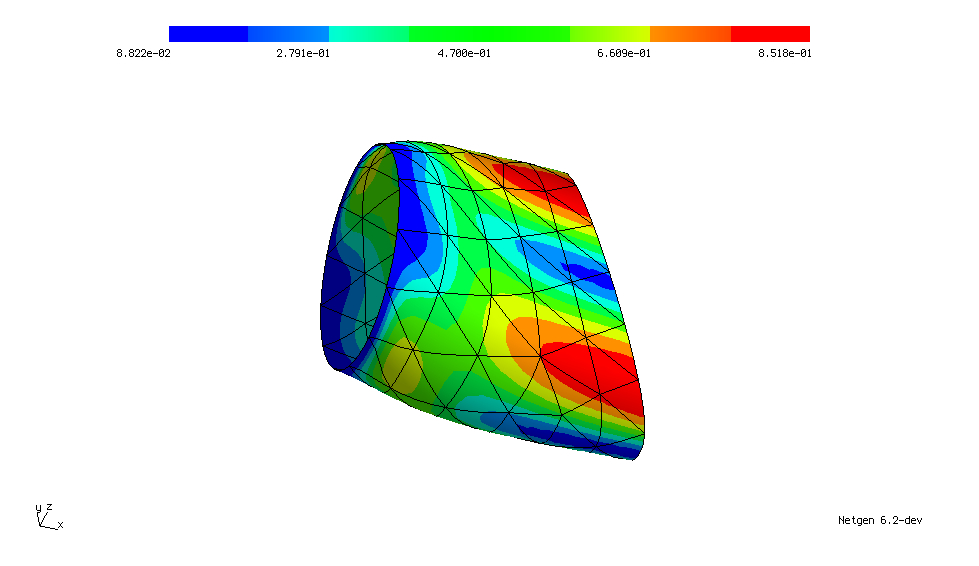
\includegraphics[width=0.6\textwidth]{../figures/naghdi.jpg}
    \caption{Naghdi shell simulation in NGSolve, solved using PETSc SNES via ngsPETSc.}
    \label{fig:ngsPETSc}
\end{figure}
%%% Put references here
\begin{thebibliography}{9.}
\frenchspacing
\bibitem{netgen}Schöberl, J., 1997. NETGEN An advancing front 2D/3D-mesh generator based on abstract rules. Computing and visualization in science, 1(1), pp.41-52.
\bibitem{ngsolve}Schöberl, J., 2014. C++ 11 implementation of finite elements in NGSolve. Institute for analysis and scientific computing, Vienna University of Technology, 30.
\bibitem{petsc}Balay, S., Abhyankar, S., Adams, M.F., Benson, S., Brown, J., Brune, P., Buschelman, K., Constantinescu, E.M., Dalcin, L., Dener, A. and Eijkhout, V., 2023. PETSc/TAO Users Manual Revision 3.19 (No. ANL-21/39). Argonne National Lab.(ANL), Argonne, IL (United States).
\bibitem{petsc4py}Dalcin, L.D., Paz, R.R., Kler, P.A. and Cosimo, A., 2011. Parallel distributed computing using Python. Advances in Water Resources, 34(9), pp.1124-1139.
\bibitem{firedrake}Rathgeber, F., Ham, D.A., Mitchell, L., Lange, M., Luporini, F., McRae, A.T., Bercea, G.T., Markall, G.R. and Kelly, P.H., 2016. Firedrake: automating the finite element method by composing abstractions. ACM Transactions on Mathematical Software (TOMS), 43(3), pp.1-27.
\end{thebibliography}
%%%%%%%%%%%%%%%%%%%%%%%%%%%%%%%%%%%%%%%%%%%%%%%%%%%%%%%%%%%%%%%%%%%%

%%% Copy and paste the above for additional talks.

\end{document}
